\chapter{Advanced Table Structure Recognition}
\label{ch:tsr_masking}

Once the foundational Layout Detection phase geometrically localizes all tabular regions within the document, the extraction methodology must resolve the grid structures. For standard, fully-ruled tables, naive parsing algorithms suffice. However, multi-modal industrial datasheets routinely embed massive, highly detailed engineering schematics, wiring graphs, or Cartesian diagrams directly within tabular cells.

This chapter details the \textit{Semantic Graph Masking} architecture developed to completely solve the debilitating phenomenon of visual hallucination in Table Structure Recognition (TSR) systems. By applying deterministic mathematical pixel obscuration, this research demonstrates the flawless utilization of the Table Transformer (TATR) backbone upon highly problematic industrial diagrams.

\section{The Core Visual Hallucination Paradigm}
\label{sec:hallucination_paradigm}

The Table Transformer (TATR) utilizes a Detection Transformer (DETR) architecture rigorously pre-trained on grid structures to decode exact row and column bounding vectors directly from image convolutions \cite{tatr}. The model does not explicitly read text; instead, it predicts structural intersections by observing physical grid lines and implicit alignment whitespace.

However, the purely visual mechanism driving TATR's success triggers catastrophic failure when processing multi-modal industrial datasheets. Consider an electrical specification table wherein the third column dynamically embeds a raster image of a wiring schematic. The schematic inherently contains thousands of high-contrast, linear graphic vectors representing wires, circuit terminals, and Cartesian testing boundaries.

WhenTATR executes inference over the parent table bounding box, its convolutional kernels identically interpret the wiring vectors as legitimate structural table boundaries. This visual interference causes TATR to aggressively over-segment the table, hallucinating hundreds of chaotic, non-existent rows within the wiring schematic to mathematically conform to the diagram's geometry. This behavior totally destroys the legitimate cross-row alignment of the true tabular data.

\section{The Semantic Pre-Masking Algorithm}
\label{sec:pre_masking_logic}

To permanently circumvent generative visual hallucination, this thesis engineers an absolute \textit{Semantic Pre-Masking} algorithm. The fundamental logic dictates that if a visual model hallucinates false rows when observing complex schematics, the mathematical tensor underlying those schematics must be erased from the observation prior to inference execution.

Instead of relying on fragile Large Language Model (LLM) instruction tuning to "ignore the graph", the intervention is purely geometrical and localized directly on the raw image array.

\subsection{Geometric Primitive Projection}
The mechanism relies on the metadata synchronization established during the initial ingestion phase. Specifically, the framework utilizes the `ImagePrimitives` array derived identically traversing the native PDF structural tree.

Let $T_{crop}$ denote the high-resolution NumPy pixel tensor array representing the structural crop of the localized Table bounding box, bounded by $B_{table} = (X_{min}, Y_{min}, X_{max}, Y_{max})$.
Let $F$ represent the set of all raster images and `Figure` bounding boxes independently identified via RT-DETR residing within the parent document.

The algorithmic algorithm mathematically projects the spatial constraints of any external figures $f_i$ directly onto the Table's localized sub-tensor. If the absolute bounding coordinates of the figure $B_{figure}$ intersect the table crop $B_{table}$, its relative localized coordinates $(x'_{min}, y'_{min}, x'_{max}, y'_{max})$ are derived dynamically:

\begin{equation}
\begin{split}
x'_{min} = \max(0, B_{figure}.x_{min} - B_{table}.x_{min}) \\
y'_{min} = \max(0, B_{figure}.y_{min} - B_{table}.y_{min})
\end{split}
\end{equation}

\begin{figure}[htbp]
\centering
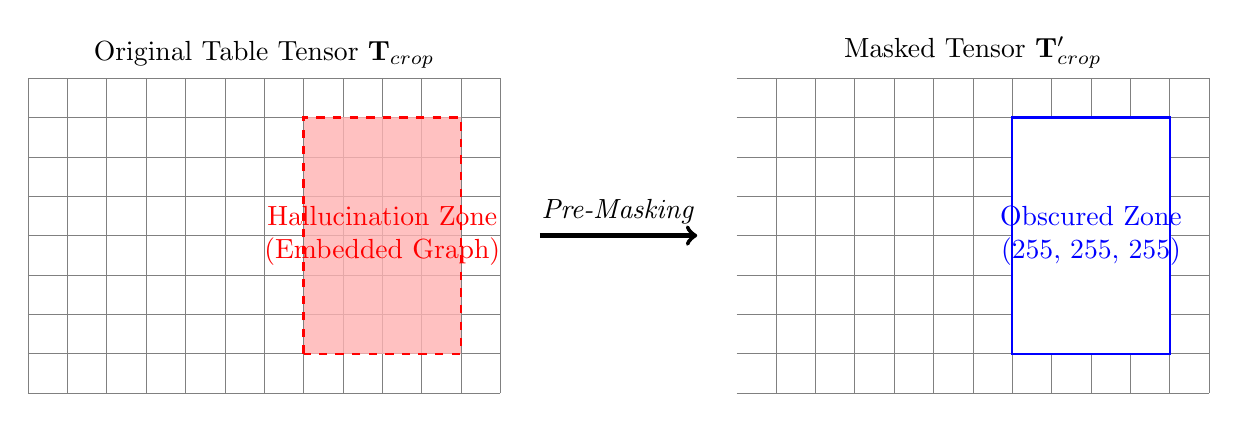
\begin{tikzpicture}[
    node distance=2.5cm,
    box/.style={rectangle, draw, thick},
]

% Background grid representing tensor
\draw[step=0.5cm,gray,very thin] (0,0) grid (6,4);
\node[above] at (3,4) {Original Table Tensor $\mathbf{T}_{crop}$};

% Sub-region for graphic
\fill[red!30, opacity=0.8] (3.5, 0.5) rectangle (5.5, 3.5);
\draw[red, thick, dashed] (3.5, 0.5) rectangle (5.5, 3.5);
\node[red, align=center] at (4.5, 2) {Hallucination Zone\\(Embedded Graph)};

% Arrows to masking
\draw[->, ultra thick] (6.5, 2) -- (8.5, 2) node[midway, above] {\textit{Pre-Masking}};

% Result grid
\draw[step=0.5cm,gray,very thin] (9,0) grid (15,4);
\fill[white] (12.5, 0.5) rectangle (14.5, 3.5);
\draw[blue, thick] (12.5, 0.5) rectangle (14.5, 3.5);
\node[blue, align=center] at (13.5, 2) {Obscured Zone\\(255, 255, 255)};
\node[above] at (12,4) {Masked Tensor $\mathbf{T}_{crop}'$};

\end{tikzpicture}
\caption{Geometric visualization of the Semantic Pre-Masking algorithm. Destructive optical obscuration totally eliminates highly-dense engineering schematic vectors prior to Table Transformer (TATR) object detection inference.}
\label{fig:semantic_masking}
\end{figure}

\subsection{Maximum-Intensity Tensor Obscuration}
Upon calculating the precise bounding parameters of the internal schematic relative to the pixel crop $T_{crop}$, the algorithm executes destructive obscuration. Utilizing optimized OpenCV geometric convolution arrays (\texttt{cv2.rectangle}), the exact tensor zone corresponding to the graphical image is blasted with maximum-intensity pixel limits $(255, 255, 255)$. 

For every sub-pixel coordinate $(x, y)$ residing within the calculated boundaries of the diagram, the original tensor intensity $T[x,y]$ is mathematically altered to true-white:

\begin{equation}
T_{crop}'(x,y) = 
\begin{cases} 
(255, 255, 255) & \text{if } x \in [x'_{min}, x'_{max}] \text{ and } y \in [y'_{min}, y'_{max}] \\
T_{crop}(x,y) & \text{otherwise}
\end{cases}
\end{equation}

\subsection{Deterministic Grid Resolution}
This mathematical intervention creates a pristine, functionally empty whitespace zone exactly where the dense engineering schematic previously resided. 

When the obscured tensor $T_{crop}'$ is evaluated dynamically by TATR, the model functions flawlessly. With the deceptive graphical vectors physically masked, the detection transformer correctly relies purely on the structural grid constraints of the remaining table to predict exact row, column, and cell coordinate lists. 

This highly localized engineering solution definitively eliminates topological table hallucination entirely independent of unreliable LLM prompting. Conclusively, it enables the integration of state-of-the-art TSR grid mapping for industrial documents, populating structurally verified topological trees directly into the unified Markdown abstraction.

\section{Unified Markdown Assembly}
\label{sec:markdown_assembly}

The entire architecture discussed across the previous chapters fundamentally converges at the final Abstract Syntax Tree (AST) compilation phase. Once RT-DETR sequences the reading order, and the Routing engine perfectly extracts text primitives and tabular \texttt{TableCell} arrays (via TATR masking or VLM XML tags), the disconnected structures must be rendered into a unified string sequence.

The pipeline achieves this by traversing the sequential geometric indices established during the XY-Cut algorithm. 
\begin{enumerate}
    \item If the topological node is classified as \texttt{Title} or \texttt{Text}, the native optical primitives are concatenated with standard newline heuristics (e.g., \texttt{\# Header} or standard paragraph returns).
    \item If the node is \texttt{Table}, the extracted \texttt{TableCell(row, col, value)} objects are algorithmically sorted and compiled into formalized Github-Flavored Markdown matrices utilizing standard vertical pipes (\texttt{|}).
    \item If the node is \texttt{Figure}, the semantic caption overriding technique detailed in Chapter 4 inserts \texttt{[TECHNICAL\_GRAPH]} placeholders.
\end{enumerate}

By adhering strictly to mathematical coordinate sequencing, the final output generated is mathematically guaranteed to reflect the complete end-to-end multi-modal ingestion of the original physical document, enabling immediate deployment into semantic Retrieval-Augmented Generation (RAG) chunking indices.
